 \documentclass[oneside]{book}
 \usepackage{epsfig,graphicx} % Required for inserting images
 \usepackage{amsmath}
 \usepackage{amsthm}
 \usepackage{amssymb}
 \usepackage{subcaption}
 \usepackage[spanish,mexico]{babel}
 \usepackage[bookmarksopen]{hyperref}
 \usepackage[utf8]{inputenc}
 \usepackage{array}
 \usepackage{listings} %Soporte para código
 \usepackage[left=2cm,right=2cm,top=1.8cm,bottom=2.3cm]{geometry}
 \usepackage{titlesec}
 \usepackage{fancyhdr} 
 \usepackage{enumitem}
 \usepackage{multicol}           % Permits header customization. See header section below.
 \usepackage{wrapfig}
 % ---definición de los paquetes--
 \fancypagestyle{plain}{
     \lhead{}
     \fancyhead[R]{\thepage}
     \fancyhead[L]{}
     \renewcommand{\headrulewidth}{0pt}
     \fancyfoot{}
 }
 \pagestyle{fancy}
 \fancyhead[R]{	hepage}
 \fancyhead[L]{}
 % Definir el tamaño del título del capítulo
 \titleformat{\chapter}[display]
   {\normalfont\huge\bfseries} % Estilo del título
   {\chaptertitlename\ \thechapter}{1pt}{\Large} % Tamaño del título
   \titlespacing*{\chapter}{0pt}{-20pt}{20pt} % Ajustar el espaciado
 
 \title{3ra lista de problemas}
 \author{Ramírez Mendoza Joaquín Rodrigo\\
 Salinas Trinidad Betsi Ivana \\
 Villalobos Juárez Gontrán Eliut\\
 Treviño Puebla Héctor Jerome}
 \date{\today}
 % ---Inicio de la portada
\begin{document}
\begin{titlepage}

	\begin{minipage}{3cm}
		\begin{center}
			
\includegraphics[height = 0.14\textheight]{recursos/Logo_UNAM.png}\par
		\end{center}
	\end{minipage}\hfill
	\begin{minipage}{10cm}

	\end{minipage}\hfill
	\begin{minipage}{3cm}
		\begin{center}
			
\includegraphics[height = 0.14\textheight]{recursos/Logo_FC.png}\par
		\end{center}
	\end{minipage}
	\centering
	\vspace{1cm}

	{\bfseries\LARGE Universidad Nacional Autónoma de México \par}

	\vspace{1cm}
	{\scshape\Large Facultad de Ciencias \par}
	\vspace{1cm}
	{\scshape\Large Matemáticas para las Ciencias Aplicadas 1 \par}
	\vspace{1cm}
	{\scshape\Large Licenciatura en Ciencias de la Computación \par}
	\vspace{1cm}
	{\scshape\Huge 3ra lista de problemas  \par}
	\vspace{3cm}
	{\itshape\Large Tercer Parcial \par}
	\vfill
	{\Large Autores: \par}
	{\Large Ramírez Mendoza Joaquín Rodrigo \par}
	{\Large Salinas Trinidad Betsi Ivana  \par}
	{\Large Villalobos Juárez Gontrán Eliut\par}
	{\Large Treviño Puebla Héctor Jerome \par}
	\vfill
	{\Large Noviembre 2024 \par}
\end{titlepage}
% ---Fin de la portada de la portada
\maketitle

% Introducir aquí sus capítulos
\chapter*{CONSTRUCCIÓN DE UNA MONTAÑA RUSA}

\textbf{1)} Un satélite se encuentra en una órbita elíptica alrededor de la Tierra. Su distancia r (en millas) desde el centro de la Tierra está dada por$$r\frac{495}{1+0.12cos\theta}$$

donde $\theta$ es el ángulo medido desde el punto de la órbita más cercano a la superficie de la Tierra (ver la figura adjunta).
\begin{enumerate}[label=\alph*)]
    \item Halla la altitud del satélite en el perigeo (el punto más cercano a la superficie de la Tierra) y en el apogeo (el punto más alejado de la superficie de la Tierra). Usa 3960 mi como el radio de la Tierra.
    \item En el instante en que $\theta$ es 120°, el ángulo $\theta$ aumenta a una tasa de 2,7° /min. Halla la altitud del satélite y la tasa a la que cambia la altitud en ese instante. Expresa la tasa en unidades de mi/min.
\end{enumerate}
\begin{center}
    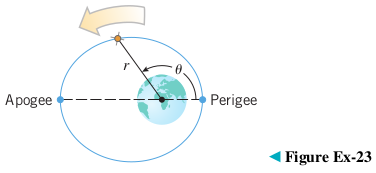
\includegraphics[height = 0.14\textheight]{recursos/image.png}\par
\end{center}

\newpage
\chapter*{ANTON-BIVENS-DAVIS 4 EJERCICIO 48}
\textbf{2)} Utilice la diferenciación implícita para demostrar que una función definida implícitamente por $sen x + cos y = 2y$ tiene un punto crítico siempre que $cos x = 0$. Luego utilice la prueba de la primera o segunda derivada para clasificar estos puntos críticos como máximos o mínimos relativos.

\begin{multicols}{2}
	\noindent
	Aplicación de la derivación implícita
	\begin{align*}
		sen (x)+cos(y)=                                                   & 2y                                      \\
		\frac{d}{dx}\left(sen (x)\right)+\frac{d}{dx}\left(cos(y)\right)= & \frac{d}{dx}\left(2y\right)             \\
		cos (x)+\left(-sen(y)\right)\frac{dy}{dx}=                        & 2\frac{dy}{dx}                          \\
		\left(-sen(y)\right)\frac{dy}{dx}-2\frac{dy}{dx}=                 & -cos (x)                                \\
		\frac{dy}{dx}\left(-sen(y)-2\right)=                              & -cos (x)                                \\
		\frac{dy}{dx}=                                                    & \frac{-cos (x)}{\left(-sen(y)-2\right)} \\
		\frac{dy}{dx}=                                                    & \frac{-cos (x)}{-\left(sen(y)+2\right)} \\
		\frac{dy}{dx}=                                                    & \frac{cos (x)}{\left(sen(y)+2\right)}   \\
	\end{align*}
	\columnbreak\\
	Análisis de púntos críticos
	\begin{align*}
		\therefore \frac{dy}{dx}= & 0\iff cos(x)=0                                          \\
		\therefore                & \text{nuestros puntos críticos ocurren en los valores:} \\
		cos(x)=                   & 0\iff x=\frac{\pi}{2}\pm k\pi, k\in\mathbb{Z}           \\
	\end{align*}
\end{multicols}
\noindent
Clasificación de los puntos críticos. Para clasificar estos puntos críticos, aplicamos la prueba de la segunda derivada.
\begin{align*}
	\frac{d^2y}{dx^2}\left(\frac{cos (x)}{sen(y)+2}\right)= & \frac{(sen(y)+2)\left(-sen(x)\right)-cos(x)\left(cos(y)\frac{dy}{dx}\right)}{\left(sen(y)+2\right)^2}         \\
	=                                                       & \frac{(sen(y)+2)\left(-sen(x)\right)-cos(x)\cdot cos(y)\cdot\frac{cos(x)}{sen(y)+2}}{\left(sen(y)+2\right)^2} \\
	=                                                       & \frac{(sen(y)+2)^2\left(-sen(x)\right)-cos^2(x)\cdot cos(y)}{\left(sen(y)+2\right)^3}
\end{align*}
Dado que la ecuación $coseno$ es periódica, toma el valor de cero en exactamente estos puntos dentro de su periodo.
$cos\left(\frac{\pi}{2}\right)=0$ y $cos\left(\frac{3\pi}{2}\right)=0$

Para ver esto más claramente:

Evaluamos los puntos donde $cos(x)=0$
\begin{align*}
	\frac{d^2y}{dx^2}\bigg|_{cos (x)=0}= & \frac{(sen(y)+2)^2\left(-sen(x)\right)-cos^2(x)\cdot cos(y)}{\left(sen(y)+2\right)^3} \\
	=                                          & \frac{(sen(y)+2)^2\left(-sen(x)\right)-0\cdot cos(y)}{\left(sen(y)+2\right)^3}                                     \\
	=                                          & -\frac{sen(x)}{\left(sen(y)+2\right)}                                          
\end{align*}
\vspace{-20px}
\begin{multicols}{2}
    Sustutuyendo en $\frac{d^2y}{dx^2}$ para $x=\frac{\pi}{2}$:
    \noindent
    \begin{align*}
        \sin\left(\frac{\pi}{2}\right) = 1 \implies \frac{d^2y}{dx^2} = -\frac{1}{\sin y + 2}
    \end{align*}
    \columnbreak\\
    Sustutuyendo en $\frac{d^2y}{dx^2}$ para $x=\frac{3\pi}{2}$:
    \begin{align*}
        \sin\left(\frac{3\pi}{2}\right) = -1 \implies \frac{d^2y}{dx^2} = \frac{1}{\sin y + 2}
    \end{align*}
\end{multicols}
\noindent
Por lo tanto, para $x = \frac{\pi}{2}+k\pi$ es negativo, lo que implica un \textbf{máximo relativo}.\\
Para $x = \frac{3\pi}{2}+k\pi$ es positivo, lo que implica un \textbf{mínimo relativo}.
\newpage
\chapter*{ANTON-BIVENS-DAVIS 9.7 EJERCICIO 29}

\textbf{29)} Encuentra los primeros 4 polinomios distintos de Taylor sobre $x = x_{0}$, y usa una utilidad gráfica para graficar la función dada y el polinomio de Taylor en la misma pantalla. \\
\begin{center}
   $f(x) = cos x$ en $  x_{0}= \pi$
\end{center}
Para facilitar la búsqueda de estos polinomios, primero hallemos las derivadas (que presentará una forma cíclica):
\begin{multicols}{3}
	\noindent
	\begin{align*}
		\text{Derivando: } &        \\
		f^{0}(x) =& cos(x) \\
        f^{1}(x) =& -sen(x) \\
        f^{2}(x) =& -cos(x) \\
        f^{3}(x) =& sen(x) \\
	\end{align*}
	\columnbreak
	\begin{align*}
		\text{Evaluando en: }& x_{0} = \pi     \\
		f^{0}(\pi) =& cos(\pi) \\
        f^{1}(\pi) =& -sen(\pi) \\
        f^{2}(\pi) =& -cos(\pi) \\
        f^{3}(\pi) =& sen(\pi) \\
	\end{align*}
	\columnbreak
	\begin{align*}
		\text{Valor: }&      \\
        cos(\pi) =& -1\\
        -sen(\pi) =&  0\\
        -cos(\pi) =&  1\\
        sen(\pi) =&   0\\
	\end{align*}
\end{multicols}
Para generar los diferestes polinomios ocuparemos el desarrollo de Taylor:
\begin{align*}
   \sum_{k=0}^{n} \frac{f^{k}(x_{0})}{k!}(x-x_{0})^{k}
\end{align*}

Para $P_{0}(x)$ :
\begin{align*}
   \sum_{k=0}^{0} \frac{f^{k}(x_{0})}{k!}(x-x_{0})^{k} &= \frac{f^{0}(\pi)}{0!}(x-\pi)^{0} \\
   \frac{f^{0}(\pi)}{0!}(x-\pi)^{0}                    &= \frac{cos(\pi)}{1}(x-\pi)^{0} \\
   \frac{cos(\pi)}{1}(x-\pi)^{0}                       &= cos(\pi)(1) \\
   cos(\pi)(1)                                         &= -1 \\
\end{align*}
Así, esta es nuestra \textbf{primera} aproximación a la función. $P_{0}(x) = -1$ \\
Para $P_{1}(x)$ :
\begin{align*}
   \sum_{k=0}^{1} \frac{f^{k}(x_{0})}{k!}(x-x_{0})^{k} &= \frac{f^{0}(\pi)}{0!}(x-\pi)^{0} + \frac{f^{1}(\pi)}{1!}(x-\pi)^{1}\\
\end{align*}
Para el nuevo Término:
\begin{align*}
   \frac{f^{1}(\pi)}{1!}(x-\pi)^{1}                    &= \frac{-sen(\pi)}{1}(x-\pi) \\
   \frac{sen(\pi)}{1}(x-\pi)                           &= sen(\pi)(x-\pi) \\
   sen(\pi)(x-\pi)                                     &= 0 \\
\end{align*}
Así la sumatoria resulta:
\begin{align*}
   \sum_{k=0}^{1} \frac{f^{k}(x_{0})}{k!}(x-x_{0})^{k} &= -1 + 0\\
   \sum_{k=0}^{1} \frac{f^{k}(x_{0})}{k!}(x-x_{0})^{k} &= -1 \\
\end{align*}
En este caso podemos ver que dada la multiplación por 0 (debido a $sen(\pi)$) el polinomio resultante es igual al anterior (NO es distinto). \\
Podremos ver que se repetirá este comportamiento siempre que el término de la sumatoria involucre  $sen(\pi)$, con esto el término se "cancelará". \\

Para $P_{2}(x)$ :
\begin{align*}
   \sum_{k=0}^{2} \frac{f^{k}(x_{0})}{k!}(x-x_{0})^{k} &= \frac{f^{0}(\pi)}{0!}(x-\pi)^{0} + \frac{f^{1}(\pi)}{1!}(x-\pi)^{1} + \frac{f^{2}(\pi)}{2!}(x-\pi)^{2}\\
\end{align*}
Para el nuevo Término:
\begin{align*}
   \frac{f^{2}(\pi)}{2!}(x-\pi)^{2}                    &= \frac{-cos(\pi)}{2}(x-\pi)^{2} \\
   \frac{-cos(\pi)}{2}(x-\pi)^{2}                      &= \frac{1}{2}(x-\pi)^{2}\\
   \frac{1}{2}(x-\pi)^{2}                              &= \frac{(x-\pi)^{2}}{2}\\
\end{align*}
Así la sumatoria resulta:
\begin{align*}
   \sum_{k=0}^{2} \frac{f^{k}(x_{0})}{k!}(x-x_{0})^{k} &= -1 + \frac{(x-\pi)^{2}}{2}\\
\end{align*}
Así, esta es nuestra \textbf{segunda} aproximación a la función. $P_{2}(x) = -1 + \frac{(x-\pi)^{2}}{2}$ \\

Para $P_{3}(x)$ :
\begin{align*}
   \sum_{k=0}^{3} \frac{f^{k}(x_{0})}{k!}(x-x_{0})^{k} &= \frac{f^{0}(\pi)}{0!}(x-\pi)^{0} + \frac{f^{1}(\pi)}{1!}(x-\pi)^{1} + \frac{f^{2}(\pi)}{2!}(x-\pi)^{2} + \frac{f^{3}(\pi)}{3!}(x-\pi)^{3}\\
\end{align*}
Para el nuevo Término: \\
Como se mecionó mas arriba sabemos que el nuevo termino involucrará a $sen(\pi)$ (Dado que la derivación de $cos(x)$ es cíclica), por esto, este término también será 0. \\
\newline
Así la sumatoria resulta:
\begin{align*}
   \sum_{k=0}^{3} \frac{f^{k}(x_{0})}{k!}(x-x_{0})^{k} &= -1 + \frac{(x-\pi)^{2}}{2} + 0\\
   \sum_{k=0}^{3} \frac{f^{k}(x_{0})}{k!}(x-x_{0})^{k} &= -1 + \frac{(x-\pi)^{2}}{2} \\
\end{align*}
Por lo tanto este no es un Polinomio Distinto. \\

Para $P_{4}(x)$ :
\begin{align*}
   \sum_{k=0}^{4} \frac{f^{k}(x_{0})}{k!}(x-x_{0})^{k} &= \frac{f^{0}(\pi)}{0!}(x-\pi)^{0} + \frac{f^{1}(\pi)}{1!}(x-\pi)^{1} + \frac{f^{2}(\pi)}{2!}(x-\pi)^{2} + \frac{f^{3}(\pi)}{3!}(x-\pi)^{3}  + \frac{f^{4}(\pi)}{4!}(x-\pi)^{4}\\
\end{align*}
Para el nuevo Término:
\begin{align*}
   \frac{f^{4}(\pi)}{4!}(x-\pi)^{4}                    &= \frac{cos(\pi)}{24}(x-\pi)^{4} \\
   \frac{cos(\pi)}{24}(x-\pi)^{4}                      &= \frac{-1}{24}(x-\pi)^{4}\\
   \frac{-1}{24}(x-\pi)^{4}                              &= -\frac{(x-\pi)^{4}}{24}\\
\end{align*}
Así la sumatoria resulta:
\begin{align*}
   \sum_{k=0}^{4} \frac{f^{k}(x_{0})}{k!}(x-x_{0})^{k} &= -1 + \frac{(x-\pi)^{2}}{2} -\frac{(x-\pi)^{4}}{24}\\
\end{align*}
Así, esta es nuestra \textbf{tercera} aproximación a la función. $P_{4}(x) = -1 + \frac{(x-\pi)^{2}}{2} -\frac{(x-\pi)^{4}}{24}$ \\

Para $P_{5}(x)$ :
\begin{align*}
   \sum_{k=0}^{3} \frac{f^{k}(x_{0})}{k!}(x-x_{0})^{k} &= \frac{f^{0}(\pi)}{0!}(x-\pi)^{0} + \frac{f^{1}(\pi)}{1!}(x-\pi)^{1} + ....  + \frac{f^{5}(\pi)}{5!}(x-\pi)^{5}\\
\end{align*}
Para el nuevo Término: \\
Este termino también involucrará a $sen(\pi)$, por esto, este término también será 0. \\
\newline
Así la sumatoria resulta:
\begin{align*}
  \sum_{k=0}^{5} \frac{f^{k}(x_{0})}{k!}(x-x_{0})^{k} &= -1 + \frac{(x-\pi)^{2}}{2} -\frac{(x-\pi)^{4}}{24} + 0\\
  \sum_{k=0}^{5} \frac{f^{k}(x_{0})}{k!}(x-x_{0})^{k} &= -1 + \frac{(x-\pi)^{2}}{2} -\frac{(x-\pi)^{4}}{24}\\
\end{align*}
Por lo tanto este no es un Polinomio Distinto. \\

Para $P_{6}(x)$ :
\begin{align*}
   \sum_{k=0}^{6} \frac{f^{k}(x_{0})}{k!}(x-x_{0})^{k} &= \frac{f^{0}(\pi)}{0!}(x-\pi)^{0} + \frac{f^{1}(\pi)}{1!}(x-\pi)^{1} + ... + \frac{f^{6}(\pi)}{6!}(x-\pi)^{6}\\
\end{align*}
Para el nuevo Término:
\begin{align*}
   \frac{f^{6}(\pi)}{6!}(x-\pi)^{6}                    &= \frac{-cos(\pi)}{720}(x-\pi)^{6} \\
   \frac{-cos(\pi)}{720}(x-\pi)^{6}                      &= \frac{1}{720}(x-\pi)^{6}\\
   \frac{1}{720}(x-\pi)^{6}                              &= \frac{(x-\pi)^{6}}{720}\\
\end{align*}
Así la sumatoria resulta:
\begin{align*}
   \sum_{k=0}^{4} \frac{f^{k}(x_{0})}{k!}(x-x_{0})^{k} &= -1 + \frac{(x-\pi)^{2}}{2} -\frac{(x-\pi)^{4}}{24} + \frac{(x-\pi)^{6}}{720}\\
\end{align*}
Así, esta es nuestra \textbf{cuarta} aproximación a la función. $P_{6}(x) = -1 + \frac{(x-\pi)^{2}}{2} -\frac{(x-\pi)^{4}}{24} + \frac{(x-\pi)^{6}}{720}$ \\
\newline
Podemos notar comportamientos similares en las aproximaciones con lo cual incluso Podríamos generar una fórmula para generar estos Polinomio. \\
\newline
\textbf{A continuación están las gráficas, tanto de la función original como de los Polinomios Generados:} \\

\begin{figure*}
    \centering
    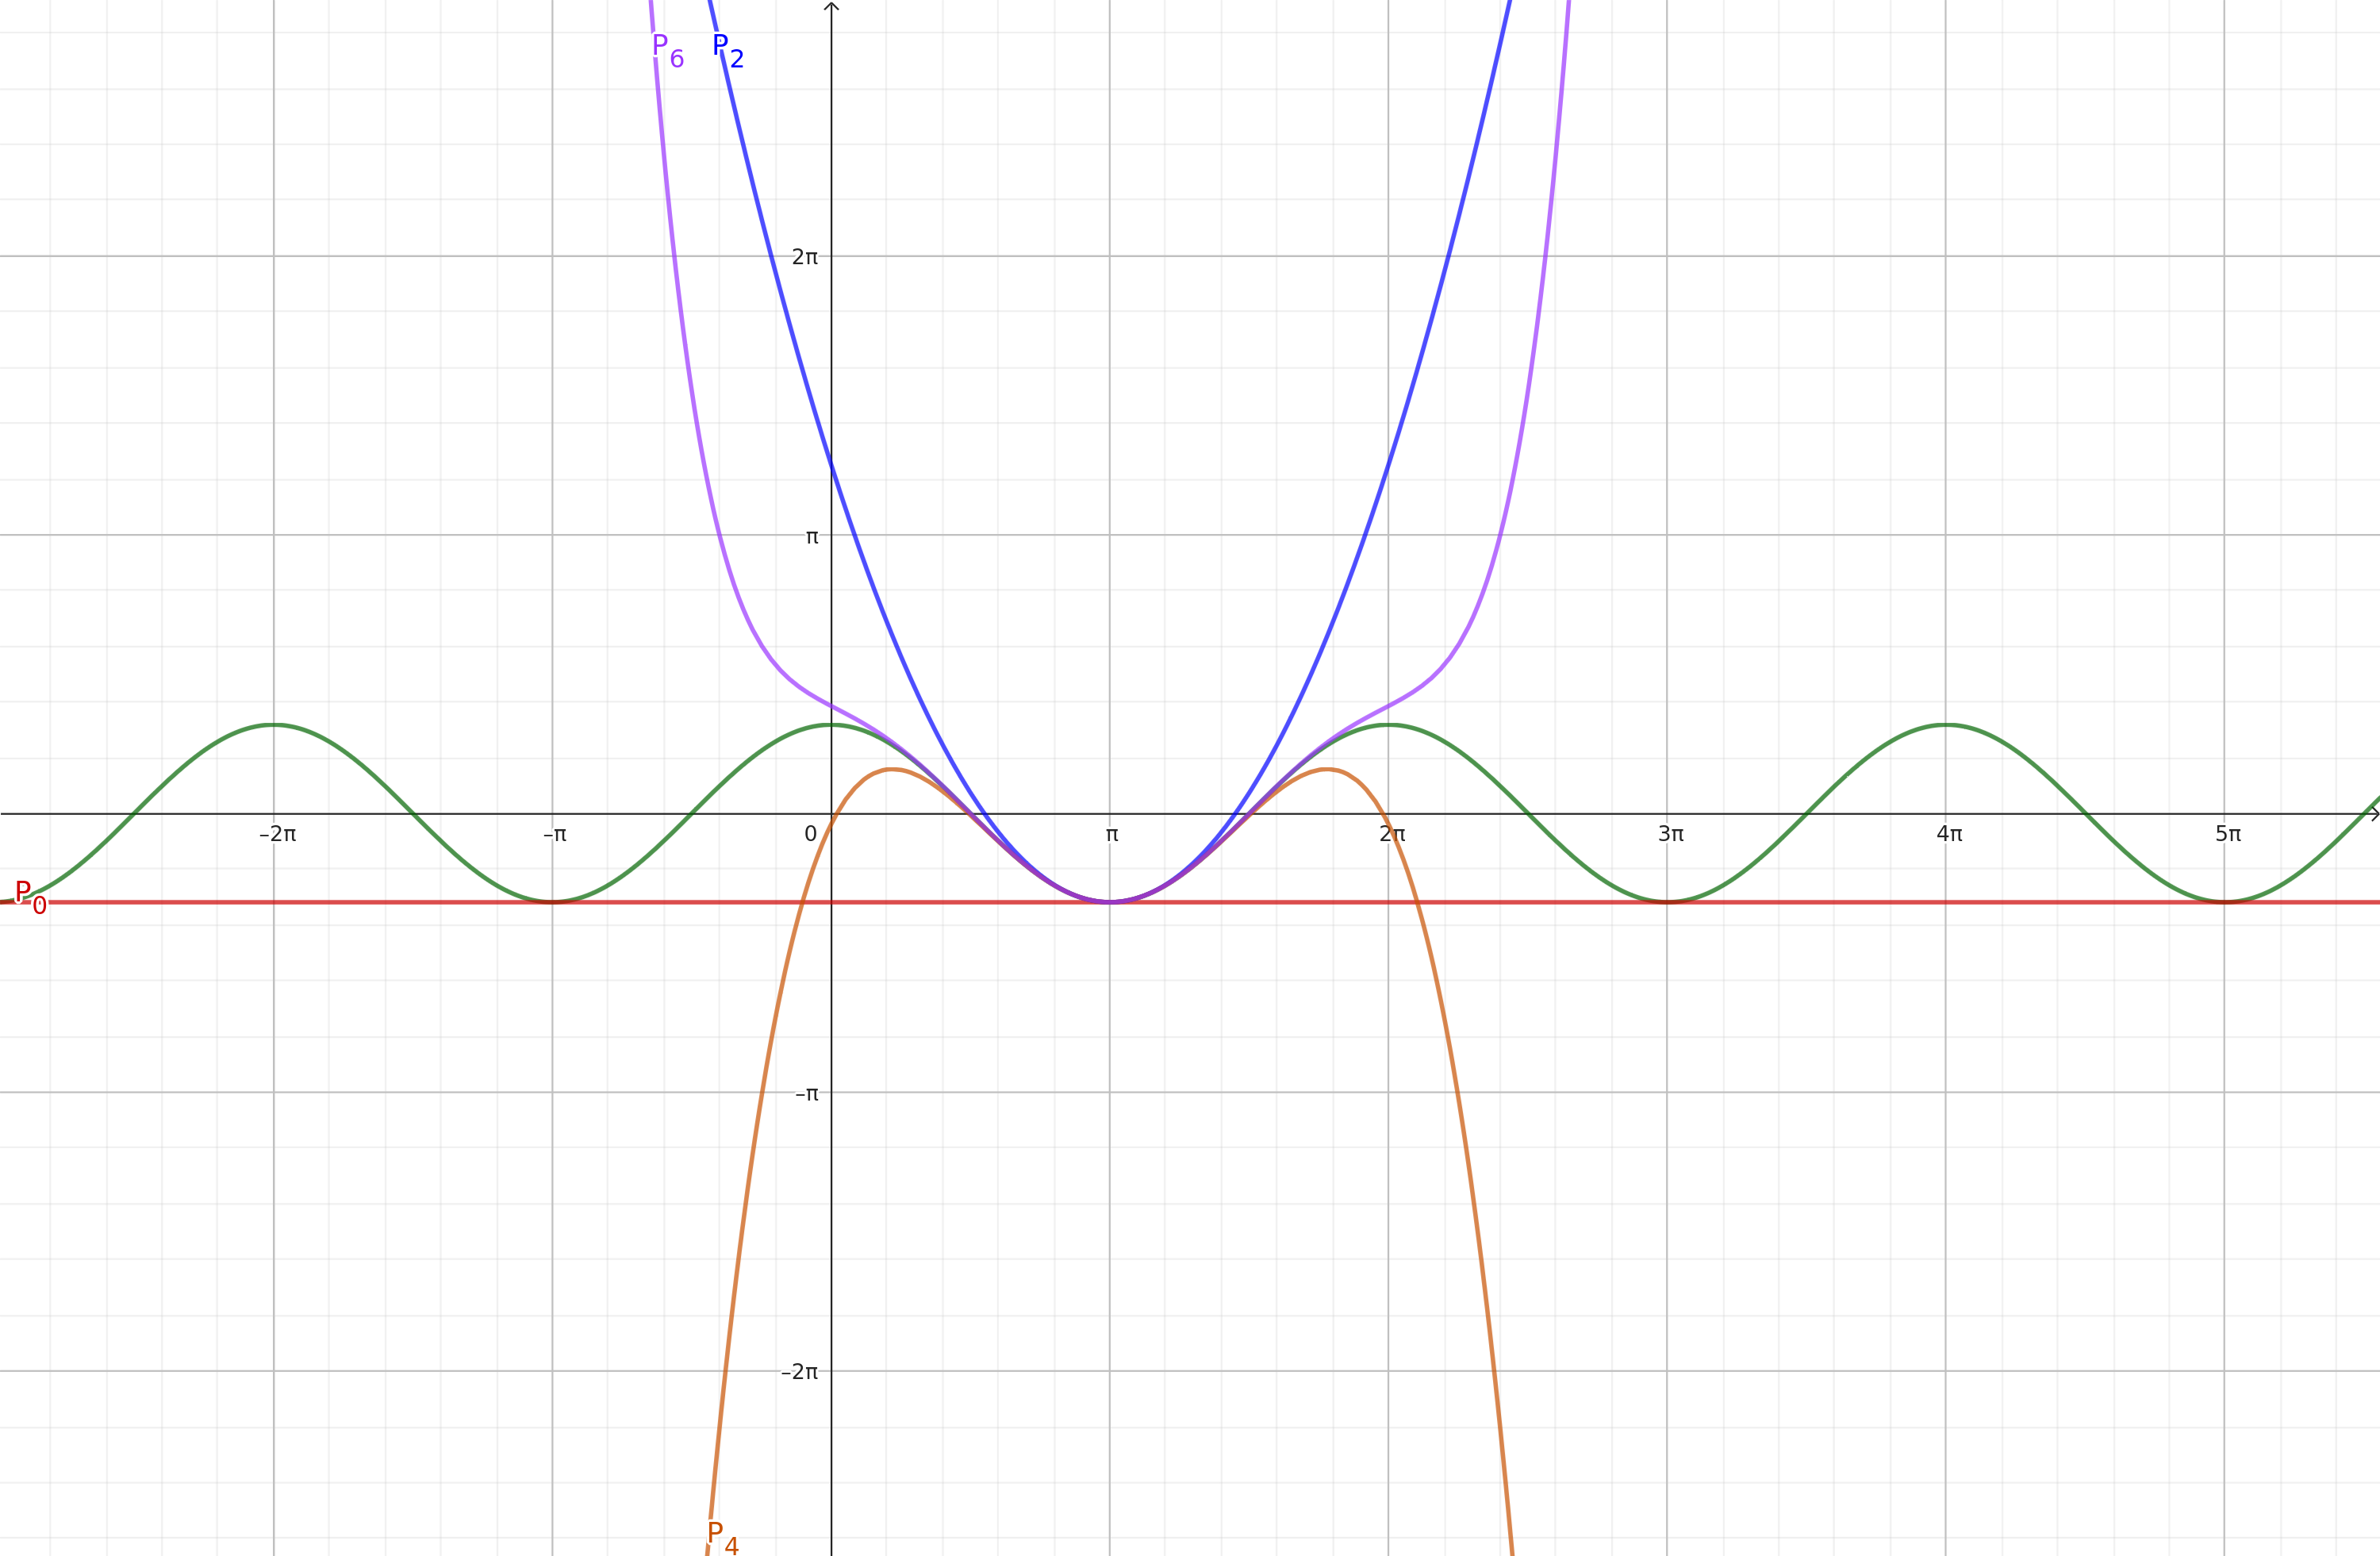
\includegraphics[height = 0.25\textheight]{recursos/polinomios/29.png}\par
    \caption*{Gráfica de la función y los Polinomios}
    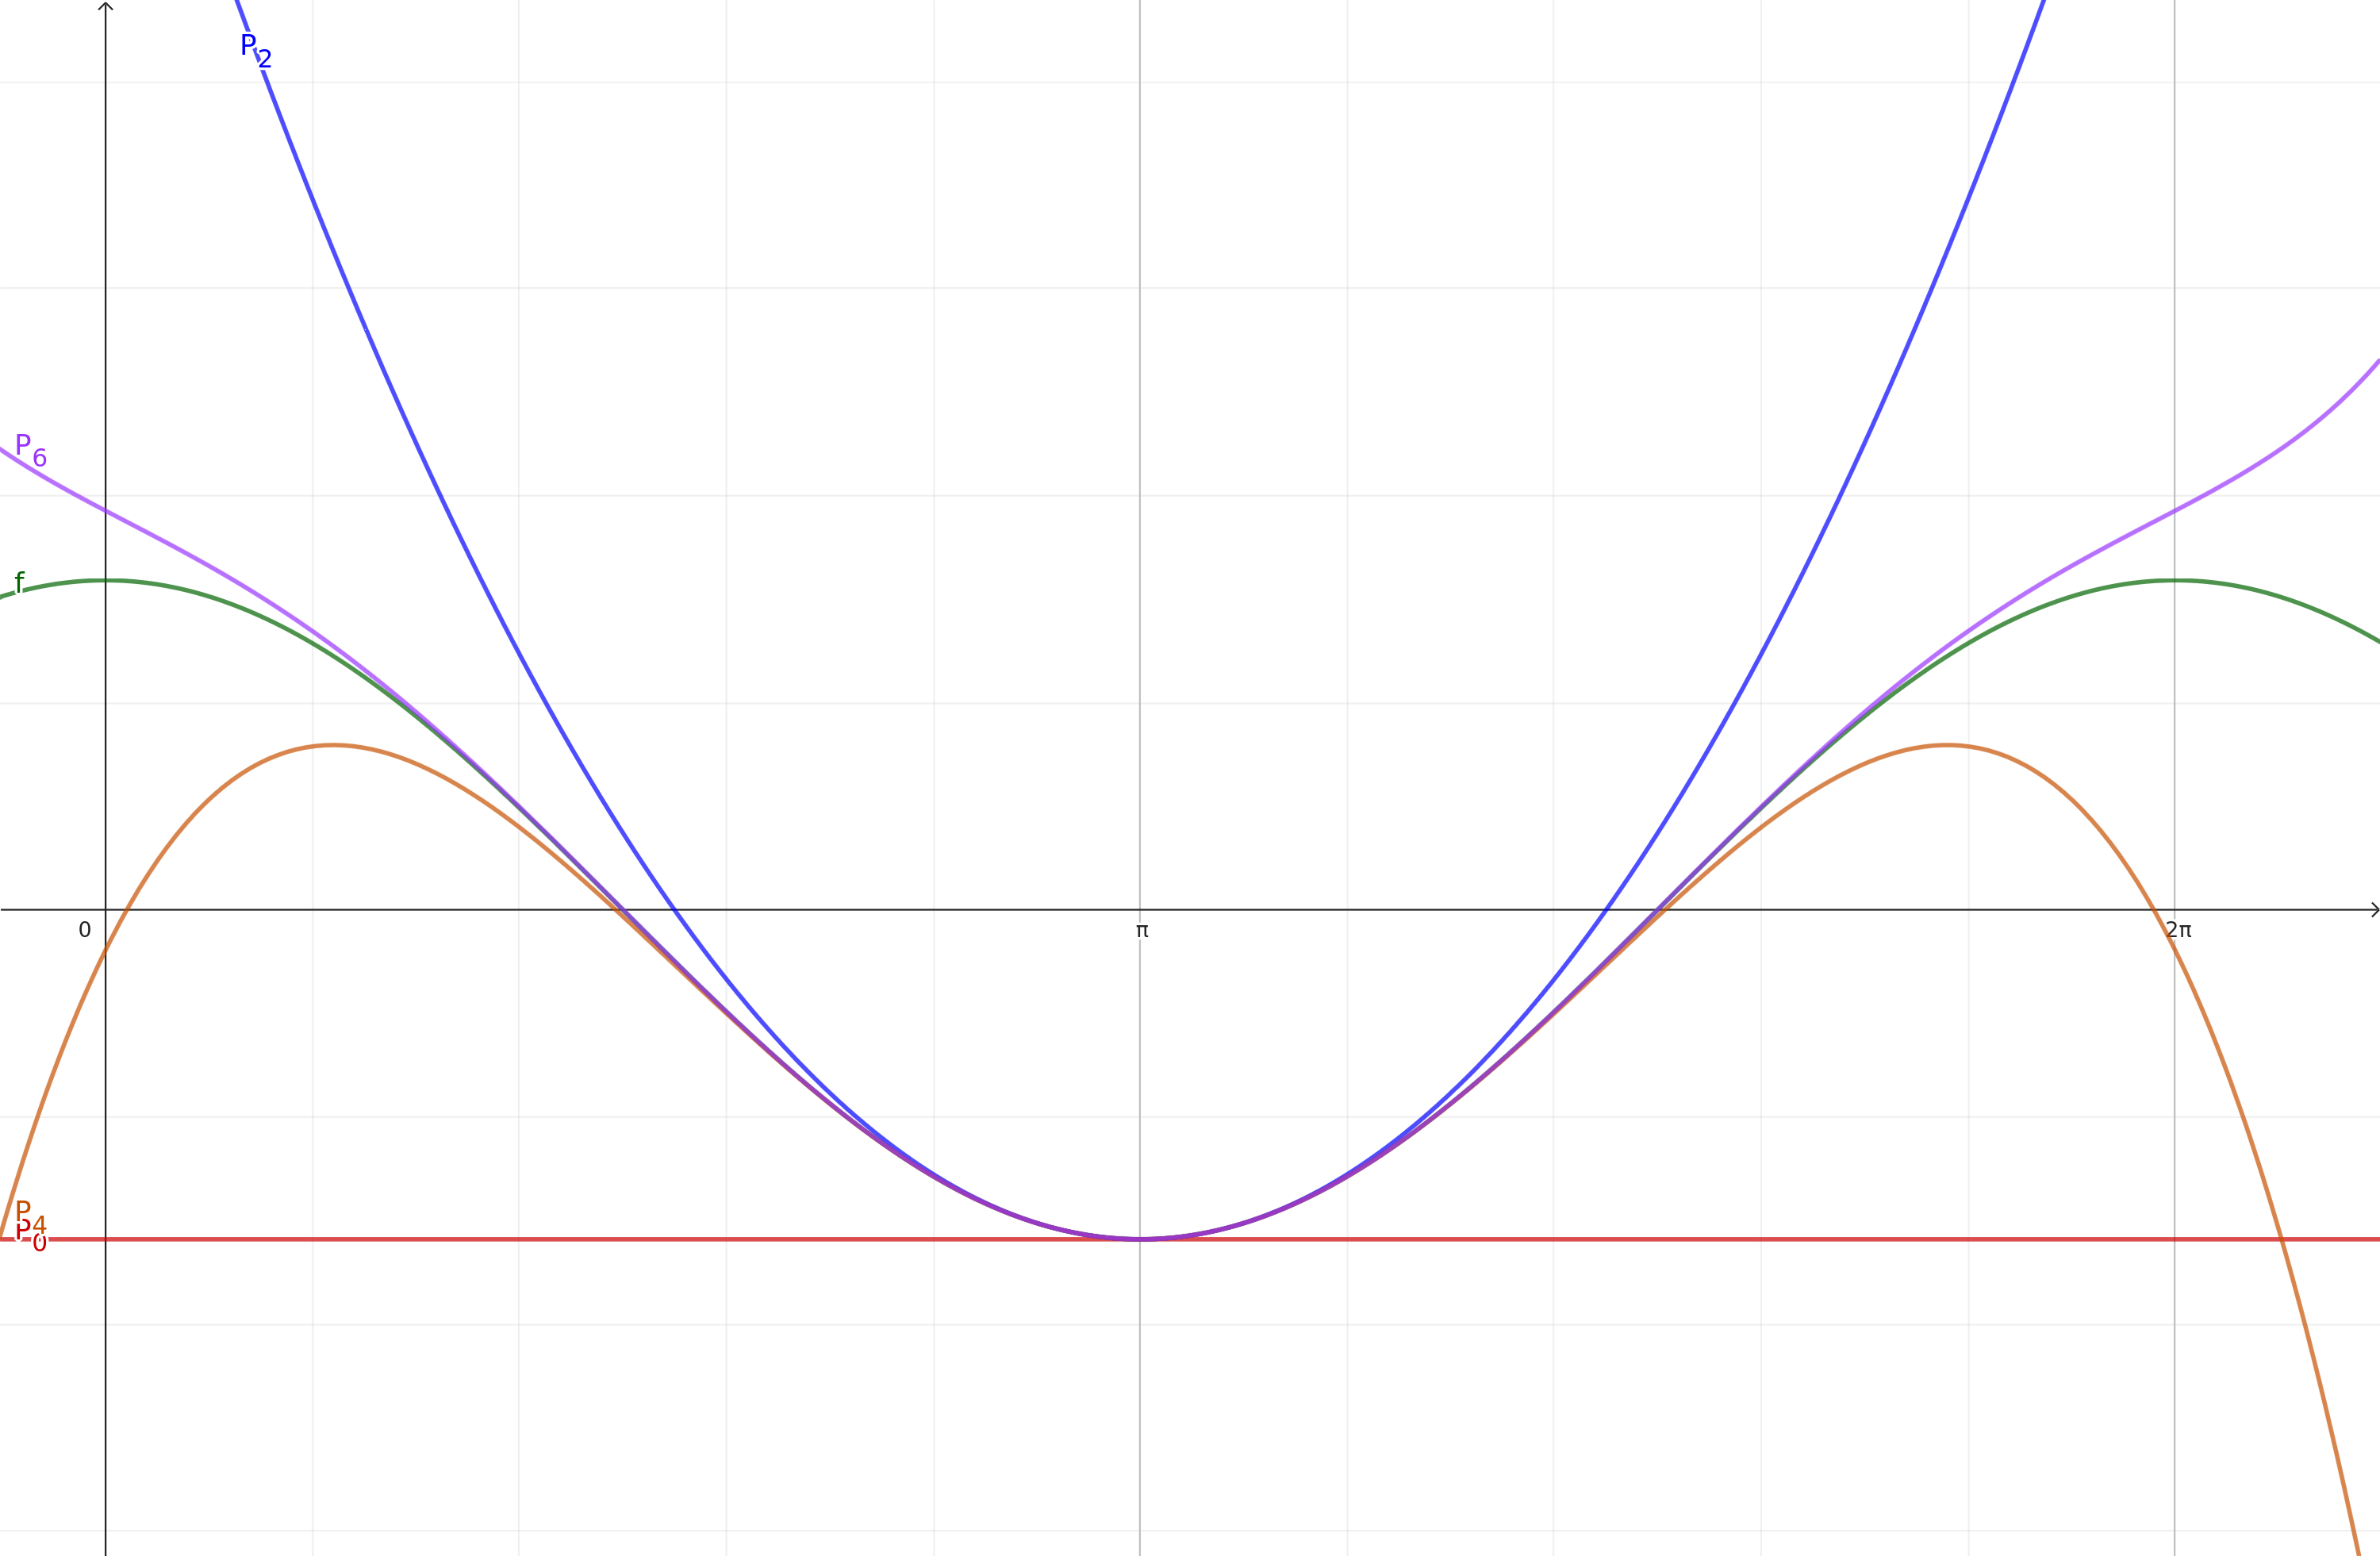
\includegraphics[height = 0.25\textheight]{recursos/polinomios/29zoom.png}\par
    \caption*{Ampliación de la Gráfica (Para notar mejor la aproximación realizada)}
    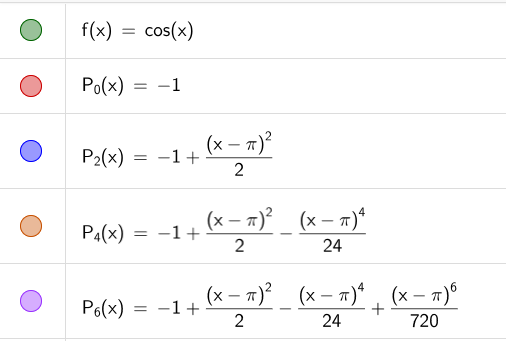
\includegraphics[height = 0.25\textheight]{recursos/polinomios/29Leyenda.png}\par
    \caption*{Simbología}
\end{figure*}

\end{document}